\documentclass[10pt,a4paper]{article}
% for margining standards
\usepackage[left=3cm,right=3cm,top=3cm,bottom=3cm]{geometry}
% for counting references as a section
\usepackage[numbib,notlof,notlot,nottoc]{tocbibind}
% useful packages
\usepackage{
                graphicx, setspace, fontspec, caption,
                subcaption, float, polyglossia, rotating,
                lscape, pdflscape, indentfirst, tocloft,
                multirow, mathtools, currfile, mathrsfs
            }
% paragraph related package
\usepackage[parfill]{parskip}
% use bzar font(THIS MUST BE LOADED BEFORE XePerian PACKAGE)
\setmainfont{BZar.ttf}
% the dear XePersian package
\usepackage{xepersian}
%
% General settings goes here.
%
% lines space
\renewcommand{\baselinestretch}{1.5}
% paragraph first line indention
\setlength{\parindent}{1cm}
% paragraph spacing
\setlength{\parskip}{1em}
% set graphics' path
\graphicspath{ {images/} }
% make table of content dotted
\renewcommand{\cftsecleader}{\cftdotfill{\cftdotsep}}
% define a new command as {half-space} in english
\newcommand{\halfspace}{\hspace{0pt}}
% define a new command as {half-space} in persian
\newcommand{\نیمفاصله}{\halfspace}
% define a shortcut for half-space in general
\renewcommand{\ }{\halfspace}
% define a new command for ease of use for rendering reference
\newcommand{\renderref}[1] { \begingroup \let\clearpage\relax \include{#1} \endgroup }
% define a shortcut for \mathscr{O}
\renewcommand{\O}{\mathscr{O}}
% define a shortcut for \mathscr{L}
\renewcommand{\L}{\mathscr{L}}
%
% DOCUMENT BEGIN
%
\begin{document}
\title{
    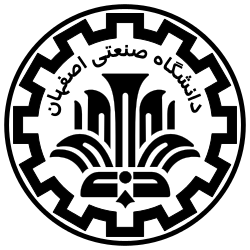
\includegraphics[width=0.25\textwidth]{iut}\\\vspace{30pt}
یادگیری ارجحیت با استفاده از انتگرال چوکت    
\\رتبه\ بندی چندجزئی    
}
\author{داریوش حسن\ پور آده}
\date{۹۳۰۸۱۶۴}
\maketitle
\null
\vfill
% make this very first page un-numbered
\thispagestyle{empty}
\setcounter{page}{0}
\newpage
در این مقاله\
\cite{THEPAPER}
در مورد یک نوع روش یادگیری ارجحیت\زیرنویس{\lr{Preference Learning}} برای رتبه\ دادن\زیرنویس{\lr{Rank}}(امتیازدهی) بین اقلام\زیرنویس{\lr{Items}} که درواقع ارجحیت دادن بین آنها می\ باشد، ارائه شده است. که وظیفه\ ی این یادگیر، یادگیری یک مدلی امتیازده است که تعدادی ورودی می\ گیرید -- که این ورودی\ ها در واقع یک (زیر)مجموعه از پیشنهادات\زیرنویس{\lr{Alternatives}} می\ باشد و خروجی این مدل ارجحیتی است که این مدل بین این پیشنهادات ورودی قائل می\ باشد. برای یادگیری مدل، مشابه آنچه که در طبقه\ بند\زیرنویس{\lr{Classifier}}ها معمول است داده\ های آموزشی به صورت نمونه\ های برچسب\زیرنویس{\lr{Labeled}} خورده استفاده می\ شود. که این برچسب\ ها در واقع ارجحیت\ های تخصیص داده شده به آن نمونه(که در واقع مجموعه\ ای از اقلام می\ باشد) هستند -- در نتیجه این روش یادگیری جز روش\ های یادگیری باناظر\زیرنویس{\lr{Supervised Learning}} می\ باشد. که به این نوع یادگیری، یادگیری رتبه\ بندی چندجزئی\زیرنویس{\lr{Multipartitle
Ranking}} می\ گویند.\بند
ایده\ ی این مقاله برای رتبه\ بندی چندجزئی این است که با استفاده از انتگرال چوکت\زیرنویس{\lr{Choquet Integral}} گسسته به عنوان یک زیرلایه مدل به عنوان تابع امتیازدهی استفاده کنیم. با این اوصاف قسمت یادگیری مدل مربوط به پیدا کردن اندازه\ گیری فازی\زیرنویس{\lr{Fuzzy Measure}}ای است که انتگرال چوکت بروی‌ آن تعریف و بنا شده است، می\ شود.\بند
این مقاله ادعا می\ کند که برای اولین با روشی برای رتبه\ بندی با استفاده از انتگرال چوکت استفاده کرده است و اینکه در مورد اینکه چرا انتگرال چوکت را به عنوان تابع ارزیاب(امتیازده) مورد استفاده قرار داده است، این است که این انتگرال را می\ توان به صورت حالت عمومی شده\ ی(تامیم داده شده\ ی) میانگین وزنی دید که علاوه بر اینکه اهمیت تک\ تک ویژگی\زیرنویس{\lr{Feature}}ها را می\ تواند استخراج کند بلکه اطلاعاتی را راجع به ارتباطات و تعاملات\زیرنویس{\lr{Interactions}} بین آن ویژگی\ ها را نیز می\ تواند استخراج کند.\بند
این مقاله مقداری در مورد کابرد انتگرال چوکت در یادگیری\ ماشین توضیحاتی مختصر داده است که بنا به دلیل اینکه خارج از موضوع این نوشتاراند از توضیح آنها صرف\ نظر می\ کنیم. سپس به شرح اندازه\ گیری\ های غیرافزودنی\زیرنویس{\lr{Non-Additive Measures}} و سپس انتگرال چوکت گسسته پرداخته است. در شرح دلیل اینکه چرا به اندازه\ گیری\ های غیرافزودنی روی آورده توضیح مفصل و روانی در مورد معایب اندازه\ گیری\ های افزودنی\زیرنویس{\lr{Additive Measures}} پرداخته است. برای ناپایداری موجود اندازه\ گیری\ های غیرافزودنی، مقاله از اندازه\ گیری\ های افزودنی استفاده کرده است.\بند
سپس مقاله به معرفی روش ارائه شده جهت یادگیری ارجحیت با استفاده از انتگرال چوکت پرداخته است؛ و تاکید داشته که نوع ارجحیت مورد بحث در مقاله از نوع رتبه\ بندی چندجزئی می\ باشد. اکثر مسائل یادگیری رتبه\ بندی، مساله\ ی یادگیری تابع رتبه\ بند\زیرنویس{\lr{Ranking Function}} می\ باشند. که زیرمجموعه\ ای همانند
$O \subset \O$
به عنوان ورودی می\ گیرد که
$\O$
به عنوان مجموعه مرجع اشیا(مثل مجموعه تمامی کتاب\ ها یا فیلم\ ها) می\ باشد. و تابع رتبه\ بند، مجموعه\ ای کاملا مرتب شده
$\preceq$
به صورت مجموعه رتبه\ بندی شده از زیرمجموعه $O$ به عنوان خروجی برمی\ گرداند. طبق آنچه که مقاله نوشته، معمولا تابع رتبه\ بند به صورت میانگین امتیازات به صورت
$U: \O \rightarrow \Re$
به طوری که
\[o \succeq o^\prime \Leftrightarrow U(o) \geq U(o^\prime)\]
که
$o, o^\prime \in \O$
؛ پرواضح است که می\ توان به تابع $U$ به عنوان درجه مطلوبیت\زیرنویس{\lr{Utility Degree}} انتصاب شده به
$o \in \O$
نگاه کرد. با درنظر گرفتن این دیدگاه، می\ توان هدف یادگیری مورد نظر را به صورت
\textit{یادگیری تابع مطلوبیت پنهان بر روی مجموعه مرجع $\O$}
تعریف کرد. که مقاله به تابع
$U(.)$\
، تابع رتبه\ بند می\ گوید؛ و همچنین این تابع دارای خاصیت ترتیب مطلق
$\prec$
می\ باشد، یعنی موارد
$U(o) = U(o^\prime)$
رخ نمی\ دهد. برای بدست آوردن تابع
$U(.)$
یک الگوریتم یادگیرنده\زیرنویس{یادگیر} همراه با داده\ های آموزشی ارائه می\ شود. به این صورت که هریک از اشیا
$o \in \O$
به یکی از کلاس\ های
$\L = \lbrace \lambda_1, \lambda_2, \ldots, \lambda_k \rbrace$
تعلق دارد، و این کلاس\ ها به\ گونه\ ای هستند که
$\lambda_1 < \lambda_2 < \ldots < \lambda_k$
. در مورد داده\ های آموزشی، شامل اشیا برچسب\ دار
$(o_i, l_i) \in \O \times \L$
که مشابه یک نمونه رگراسیون معمولی می\ باشند.\\
همانطور که قبلا هم گفته شد هدف یادگیری تابع رتبه\ بند
$U(.)$
می\ باشد به\ طوری که با چیدمان کلاس\ ها سازگار باشد به\ گونه\ ای که اشیاءای که به کلاس\ های بالاتر(در رابطه\ ی ترتیب کلاس\ ها) تعلق داشته باشند دارای رتبه\ ی بالاتری نسبت به اشیاء متعلق به کلاس\ های پایین\ تر باشند. -- در مورد توضیح مسائل رتبه\ بندی کلاس\ ها بنابه محدودیت موجود در تعداد صفحات این نوشتار، تا به اینجا اکتفا می\ کنم.\بند
در مورد اینکه در این جریان، جایگاه انتگرال چوکت در مساله یادگیری رتبه\ بند در کجاست؟ می\ توان گفت که ایده\ ی این مقاله این است که نمایش تابع مطلوبیت پنهان
$U(.)$
از انتگرال چوکت استفاده کرده است. با این فرض که اشیا
$o \in \O$
به صورت برداری از ویژگی\ ها نمایش داده می\ شود.
\begin{equation}
f_o = (f_o(x_1), \ldots, f_o(x_n))
\label{fo}
\end{equation}
که رابطه\ ی
\ref{fo}
را می\ توان به عنوان ارزیابی که از شی $o$ نسبت به معیارهای(کلاس\ ها) $x_i$ دارد، می\ باشد. پس طبق فلسفه\ ی انتگرال\ فازی که ترکیب اطلاعات منابع اطلاعاتی\ مان با توجه به اهمیت آنها می\ باشد می\ توان تابع درجه\ ی مطلوبیت $U(.)$ را به صورت
\ref{uo}
تعریف کرد.
\begin{equation}
U(o) =  \zeta_\mu(f_o)
\label{uo}
\end{equation}
که در رابطه\ ی
\ref{uo}
نماد
$\zeta_\mu$،
انتگرال چوکت می\ باشد.\بند
این مقاله\
\cite{THEPAPER}
موضوع بسیار جالبی را با نوشتاری بسیار گویا و روان شرح داده که برای موضوع سمینار این درس مناسب می\ باشد؛ که متاسفانه به علت محدودیت صفحاتی این نوشتار بیشتر نمی\ توان توضیح داد.
\vspace{10pt}\\
{\LARGE مرجع}
\nocite{*}
\renderref{reference}
\end{document}
